% A simple commutative diagram
% Stefan Kottwitz
\documentclass{article}
\usepackage{tikz}
\usepackage{amsmath}
\usetikzlibrary{matrix}
\begin{document}
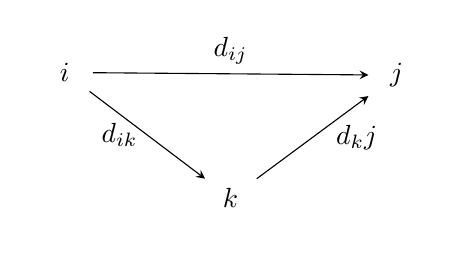
\begin{tikzpicture}
  \matrix (m) [matrix of math nodes,%
    row sep=3em,column sep=4em,minimum width=2em]
  {
     i &   &j \\
       & k &  \\};
  \path[-stealth]
    (m-1-1) edge node [left] {$d_{ik}$} (m-2-2)
            edge node [above] {$d_{ij}$} (m-1-3)
    (m-2-2) edge node [right=0.5em,dashed,-] {$d_kj$}(m-1-3);

\end{tikzpicture}
\end{document}
